\section*{Results}

\subsection*{Example of work}

\begin{center}
    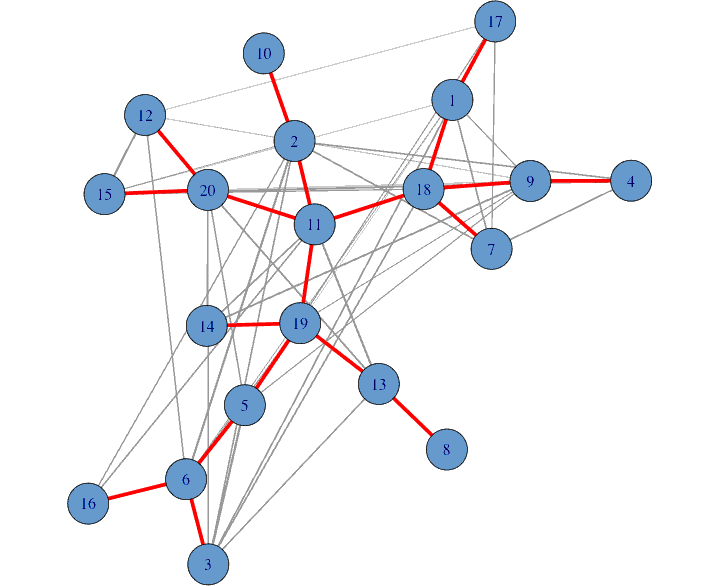
\includegraphics[width=0.6\linewidth]{../results/mst.png}
    \captionof{figure}{Minimum spanning tree}
    \label{fig_rho_1_all}
\end{center}


\subsection*{Execution time analysis}
The described algorithms and their modifications was tested on graphs with different size and density.

\begin{center}
    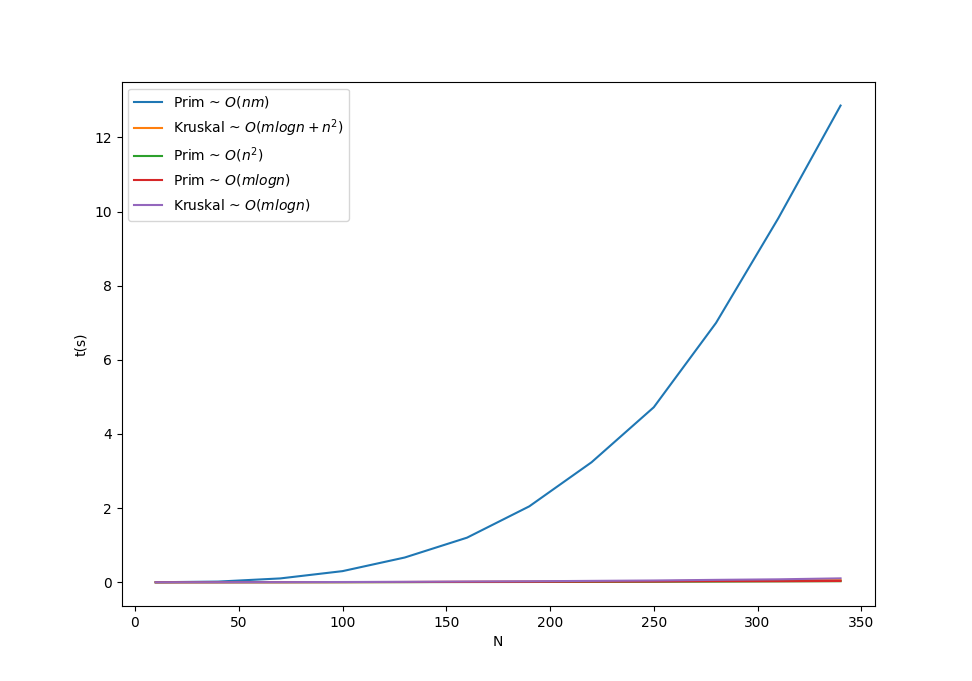
\includegraphics[width=0.75\linewidth]{../results/rho_1_all.png}
    \captionof{figure}{Execution time on dense graphs with $\rho = 1$}
    \label{fig_rho_1_all}
\end{center}

\begin{center}
    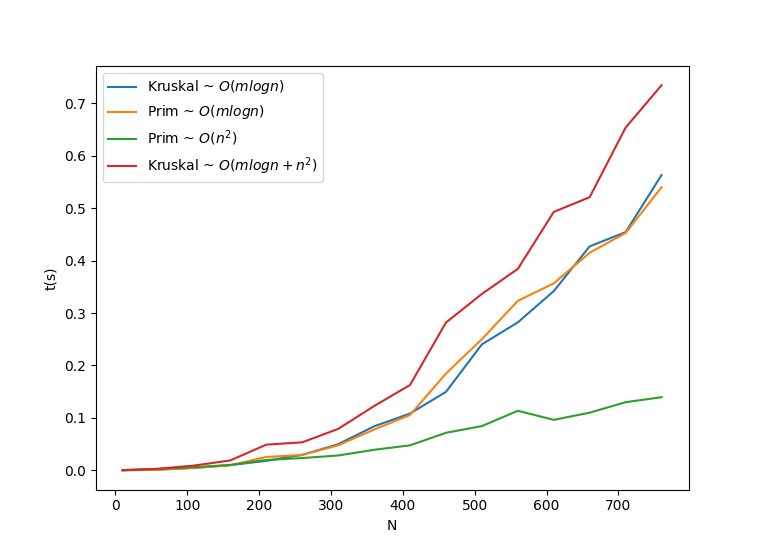
\includegraphics[width=0.75\linewidth]{../results/rho_1_fast.png}
    \captionof{figure}{Execution time on dense graphs with $\rho = 1$}
    \label{fig_rho_1_fast}
\end{center}


From Figure \ref{fig_rho_1_all} it can be seen that execution time of base Prim algorithm is significantly higher than others as it has the highest complexity among others algorithms.

From Figure \ref{fig_rho_1_fast} it can be seen that the best time is observed for Prim algorithm for dense graphs. As for complete graphs the number of edges $m = \frac{n(n - 1)}{2}$, thus other algorithms with complexity depends on $m$ it is higher than $n^2$.

\begin{center}
    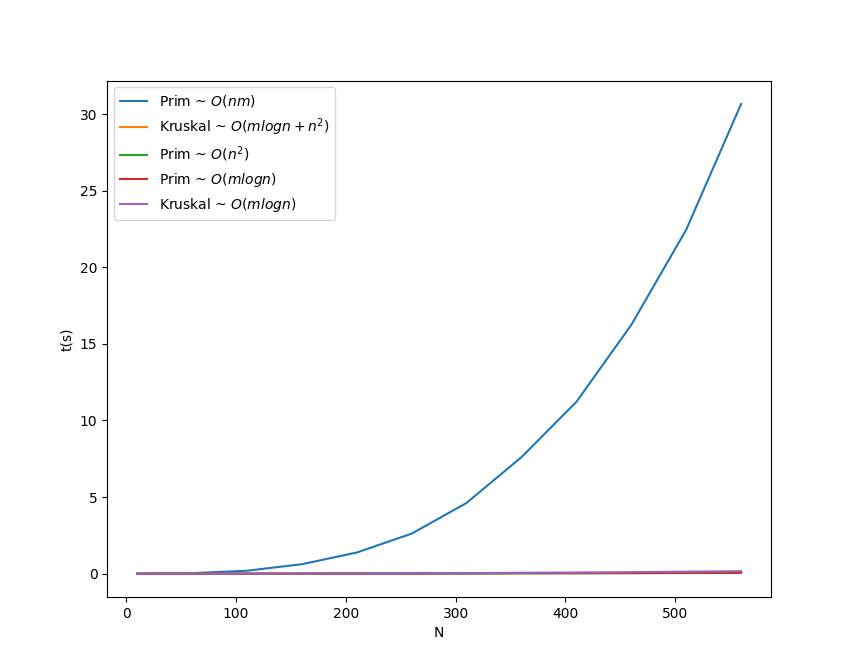
\includegraphics[width=0.75\linewidth]{../results/rho_0.5_all.png}
    \captionof{figure}{Execution time on graphs with $\rho = 0.5$}
    \label{fig_rho_0.5_all}
\end{center}

\begin{center}
    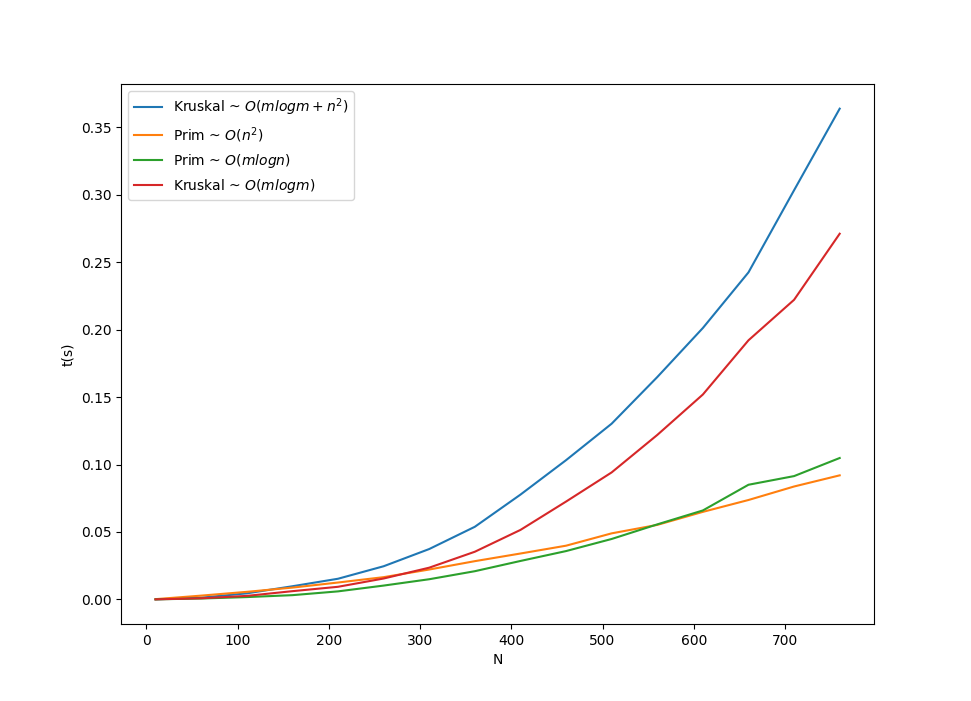
\includegraphics[width=0.75\linewidth]{../results/rho_0.5_fast.png}
    \captionof{figure}{Execution time on graphs with $\rho = 0.5$}
    \label{fig_rho_0.5_fast}
\end{center}

From Figure \ref{fig_rho_0.5_fast} we can notice next things:

\begin{itemize}
    \item the difference between Prim algorithm with $O(n^2)$ and others became less
    \item on the small (< 550 vertices) graphs sparse Prim algorithm works better, although with growth of vertices (and therefore edges) the dense  algorithm becomes faster. 
\end{itemize}

\begin{center}
    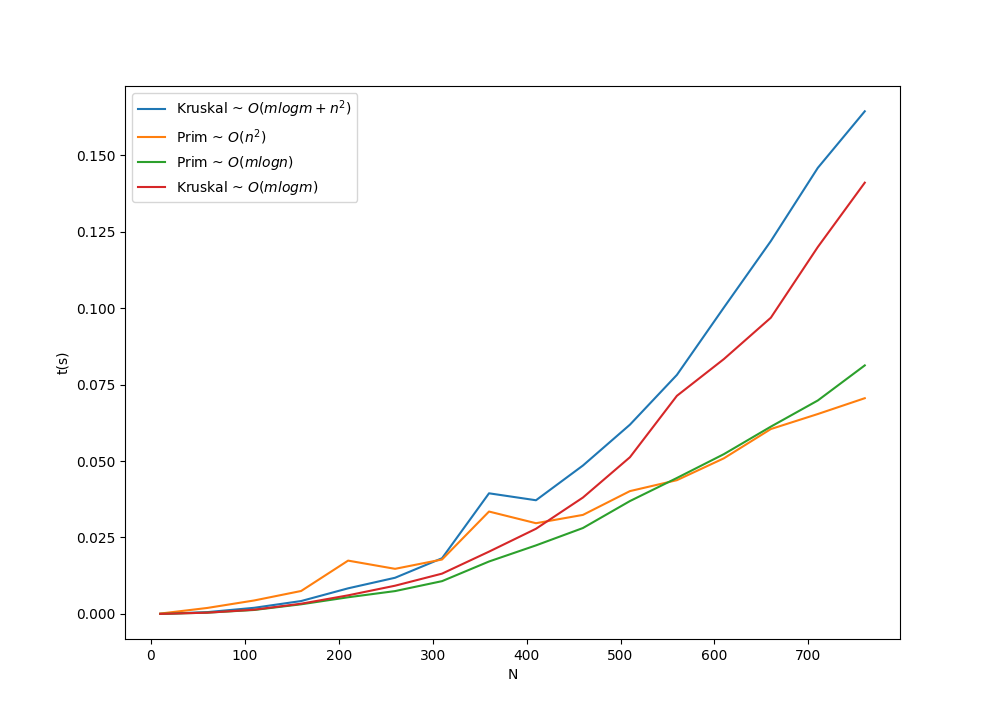
\includegraphics[width=0.75\linewidth]{../results/rho_0.25_fast.png}
    \captionof{figure}{Execution time on graphs with $\rho = 0.25$}
    \label{fig_rho_0.25_fast}
\end{center}

\begin{center}
    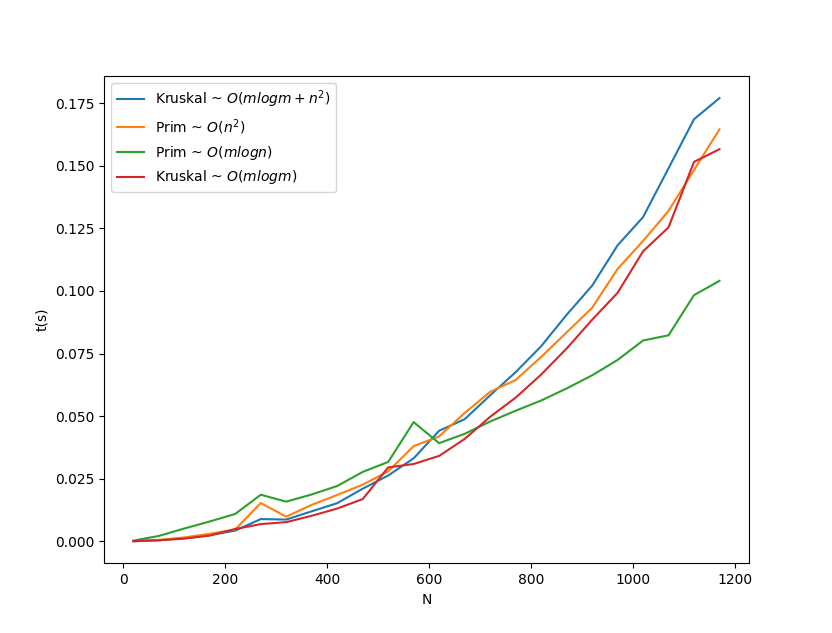
\includegraphics[width=0.75\linewidth]{../results/rho_0.1_fast.png}
    \captionof{figure}{Execution time on graphs with $\rho = 0.1$}
    \label{fig_rho_0.1_fast}
\end{center}

\begin{center}
    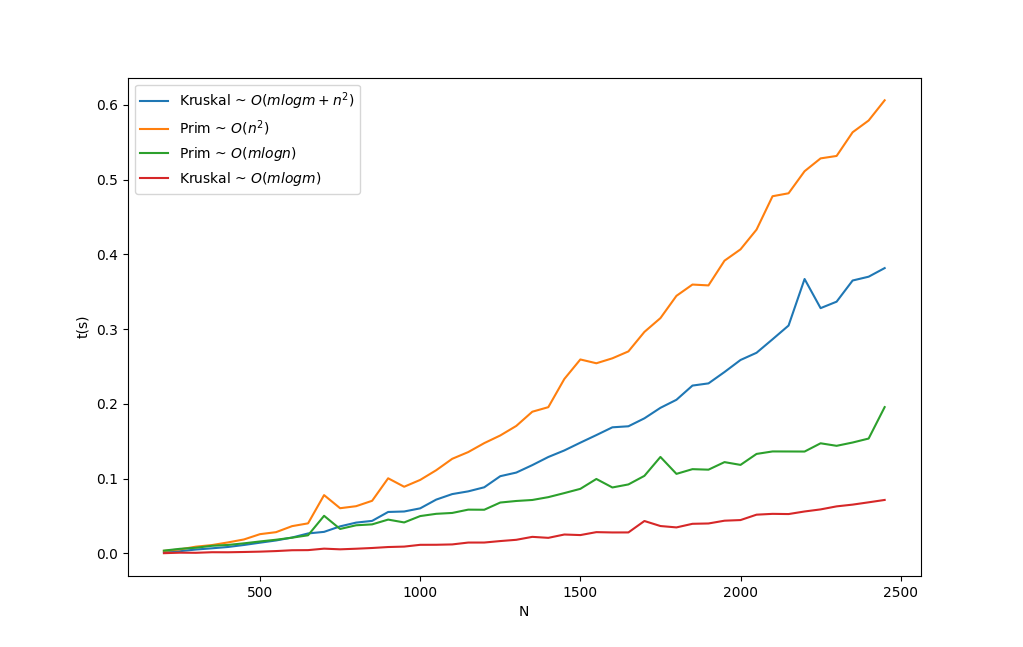
\includegraphics[width=0.75\linewidth]{../results/rho_0.05.png}
    \captionof{figure}{Execution time on graphs with $\rho = 0.05$}
    \label{fig_rho_0.05}
\end{center}

From figures \ref{fig_rho_0.25_fast}, \ref{fig_rho_0.1_fast}, \ref{fig_rho_0.05} we can see that with the decreasing of density the dense Prim algorithm becomes slower than other modifications.
As well as that can be seen that while having higher (than sparse Prim) complexity, Kruskal algorithm shows better results on the small density graphs ($\rho=0.005$).
It can be explained by the fact that on low density the number of edges $m$ goes to number of vertices $n$ and thats why Kruskal complexity $O(mlogm)$  goes similar to sparse Prim complexity $O(mlogn)$ which in fact goes to $O(n log n)$.
It can be seen from the last figure that Kruskal DSU and sparse Prim algorithms have similar level of growth, while the difference in time, probably, can be explained by lower constant for particular implementation of Kruskal algorithm.

